%%
%% This is file `sample-sigconf.tex',
%% generated with the docstrip utility.
%%
%% The original source files were:
%%
%% samples.dtx  (with options: `sigconf')
%% 
%% IMPORTANT NOTICE:
%% 
%% For the copyright see the source file.
%% 
%% Any modified versions of this file must be renamed
%% with new filenames distinct from sample-sigconf.tex.
%% 
%% For distribution of the original source see the terms
%% for copying and modification in the file samples.dtx.
%% 
%% This generated file may be distributed as long as the
%% original source files, as listed above, are part of the
%% same distribution. (The sources need not necessarily be
%% in the same archive or directory.)
%%
%% The first command in your LaTeX source must be the \documentclass command.
\documentclass[sigconf]{acmart}

%%
%% \BibTeX command to typeset BibTeX logo in the docs
\AtBeginDocument{%
  \providecommand\BibTeX{{%
    \normalfont B\kern-0.5em{\scshape i\kern-0.25em b}\kern-0.8em\TeX}}}

%% Rights management information.  This information is sent to you
%% when you complete the rights form.  These commands have SAMPLE
%% values in them; it is your responsibility as an author to replace
%% the commands and values with those provided to you when you
%% complete the rights form.
\setcopyright{acmcopyright}
\copyrightyear{2024}
\acmYear{2024}
%\acmDOI{10.1145/1122445.1122456}

%% These commands are for a PROCEEDINGS abstract or paper.
\acmConference[ASD24/25]{The first project delivery of ASD24/25}{2024}{Faculdade de Ciências e Tecnologia, NOVA University of Lisbon, Portugal}
\acmBooktitle{The Projects of ASD - first delivery, 2024, Faculdade de Ciências e Tecnologia, NOVA University of Lisbon, Portugal}
%\acmPrice{15.00}
%\acmISBN{978-1-4503-XXXX-X/18/06}

\usepackage{algorithm}
\usepackage{algpseudocode}
\usepackage{afterpage}
\usepackage{lipsum}
\usepackage{multicol}
\usepackage{pgfplots}
\pgfplotsset{compat=1.18}
\usepackage{tikz}
\usetikzlibrary{arrows.meta, positioning, calc}
%%
%% Submission ID.
%% Use this when submitting an article to a sponsored event. You'll
%% receive a unique submission ID from the organizers
%% of the event, and this ID should be used as the parameter to this command.
%%\acmSubmissionID{123-A56-BU3}

%%
%% The majority of ACM publications use numbered citations and
%% references.  The command \citestyle{authoryear} switches to the
%% "author year" style.
%%
%% If you are preparing content for an event
%% sponsored by ACM SIGGRAPH, you must use the "author year" style of
%% citations and references.
%% Uncommenting
%% the next command will enable that style.
%%\citestyle{acmauthoryear}


%%
%% end of the preamble, start of the body of the document source.
\begin{document}
%%
%% The "title" command has an optional parameter,
%% allowing the author to define a "short title" to be used in page headers.
\title{Distributed Systems Algorithms - Distributed Ledger}

%%
%% The "author" command and its associated commands are used to define
%% the authors and their affiliations.
%% Of note is the shared affiliation of the first two authors, and the
%% "authornote" and "authornotemark" commands
%% used to denote shared contribution to the research.
\author{Gonçalo Virgínia}
\authornote{Student number 56773}
\email{g.virginia@campus.fct.unl.pt}
\affiliation{%
  \institution{MIEI, DI, FCT, UNL}
}

\author{Ricardo Rodrigues}
\authornote{Student number 72054}
\email{rf.rodrigues@campus.fct.unl.pt}
\affiliation{%
  \institution{MEI, DI, FCT, UNL}
}

%%
%% By default, the full list of authors will be used in the page
%% headers. Often, this list is too long, and will overlap
%% other information printed in the page headers. This command allows
%% the author to define a more concise list
%% of authors' names for this purpose.
\renewcommand{\shortauthors}{G. Virgínia, R. Rodrigues}

%%
%% The abstract is a short summary of the work to be presented in the
%% article.
\begin{abstract}
    Distributed ledgers (DLTs) are decentralized databases maintained and updated across multiple nodes in a distributed system, relying on consensus algorithms to ensure agreement, ordering of events, and synchronization among participants - combating potential failures or inconsistencies in the network, and, most importantly, eliminating the need for centralized coordination. \\
    This makes DLTs suitable for a wide range of applications, including data sharing, asset tracking, and collaborative systems. Nonetheless, although this approach offers robustness and fault tolerance, it naturally also presents its own challenges with respect to latency, throughput, and scalability, which can be mitigated through multiple approaches. \\
    To this end, this project employs two different approaches consisting of mainstream consensus algorithms: the relatively simple ABD Quorum, and, a more complex State Machine + Multi-Paxos stack (with two Multi-Paxos variants: Classic, and Distinguished Learner). \\
\end{abstract}


%%
%% This command processes the author and affiliation and title
%% information and builds the first part of the formatted document.
\maketitle

\section{Introduction}

The following sub-sections describe the abstracted ideas for both previously mentioned approaches.

\subsection{ABD Quorum}

The ABD Quorum algorithm is a relatively protocol for maintaining consistency and fault tolerance, by ensuring that both read and write operations are performed reliably by requiring a majority quorum of replicas to participate. A write operation involves sending a value, along with a unique "timestamp" - or "tag" consisting of an (opSeq, processId) tuple - to all other replicas. Each replica updates its stored value and timestamp only if the incoming write is more recent. For a read operation, a client queries a quorum of replicas to determine the most up-to-date value based on the highest timestamp/tag. Finally, the replica originally contacted by the client then propagates this value to ensure it is written back to the replicas, maintaining consistency.

Operation "timestamp" (Tag) comparisons take the following form: <s1, i1> > <s2, i2> if s1 > s2 or (s1 = s2 and i1 > i2) - meaning, the operation sequence number always takes precedence in terms of importance, as would be expected, but, in the case of two operations have the same opSequence number, the highest process ID wins the transaction. 

The algorithm relies on these intersections between read and write quorums to guarantee that the most recent data is always accessible, preventing stale reads. This method is ensured to work as long as a quorum receives replies from (numReplicas / 2) + 1 replicas, given that, at the bare minimum, a valid subsequent quorum will intersect at least 1 replica from the previous quorum, which will contain the most up-to-date value. \\

As expected, the protocol stack is fairly trivial - consisting solely of the ABD Quorum protocol for both replication and consistency of the Application's state: \\

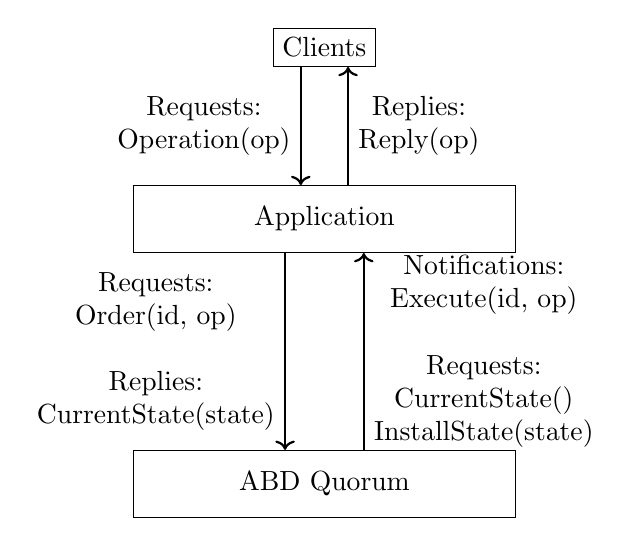
\begin{tikzpicture}[]  
    \node (clients) [draw, rectangle, minimum width=0.1\textwidth, minimum height=0.04\textwidth] {Clients};
    \node (app) [draw, rectangle, below=1.5 of clients, minimum width=0.4\textwidth, minimum height=0.07\textwidth] {Application};
    \node (repl) [draw, rectangle, below=2.5 of app, minimum width=0.4\textwidth, minimum height=0.07\textwidth] {ABD Quorum};

   \draw[->, thick] (clients.south) ++(-0.3, 0) -- ++(0,-1.5) node[midway, left, align=center] {Requests: \\ Operation(op)};
   \draw[<-, thick] (clients.south) ++(0.3,0) -- ++(0,-1.5) node[midway, right, align=center] {Replies: \\ Reply(op)};

   \draw[->, thick] (app.south) ++(-0.5, 0) -- ++(0,-2.5) node[midway, left, align=center] {Requests: \\ Order(id, op) \\  \\ Replies: \\ CurrentState(state)};
   \draw[<-, thick] (app.south) ++(0.5,0) -- ++(0,-2.5) node[midway, right, align=center] 
    {Notifications: \\ Execute(id, op) \\ \\ Requests: \\ CurrentState() \\ InstallState(state)};
\end{tikzpicture} \\

Clients send their requests to the Application layer, whose sole job is to send operations down to the ABD Quorum algorithm, for both replicating writes, and maintaining the most up-to-date state for any read - consequently, after an operation passes a majority of replicas via the ABD protocol, a reply is sent upwards, confirming the execution of a given operation, and thus, updating the Application's state - which, finally, enables a correct reply to the original client.

\subsection{State Machine + Multi-Paxos}

The State Machine Replication (SMR) protocol is responsible for managing the execution and replication of client operations within the distributed system. It handles client requests by ensuring their operations are replicated and ordered consistently through the agreement protocol. The SMR tracks the sequence of commands, determines the decided operations for each position in the sequence, and notifies the application to execute these operations in the correct order.

Additionally, the protocol oversees the communication channel, including maintaining open TCP connections and managing membership changes in the system. This involves facilitating the addition of new replicas to the replica set, notifying the agreement protocol about membership updates, and detecting replica failures. Upon detecting a failure, the SMR protocol attempts to reconnect with the failed replica a configurable number of times. If the replica is deemed non-functional, the protocol issues a state machine operation to remove it from the replica set. \\

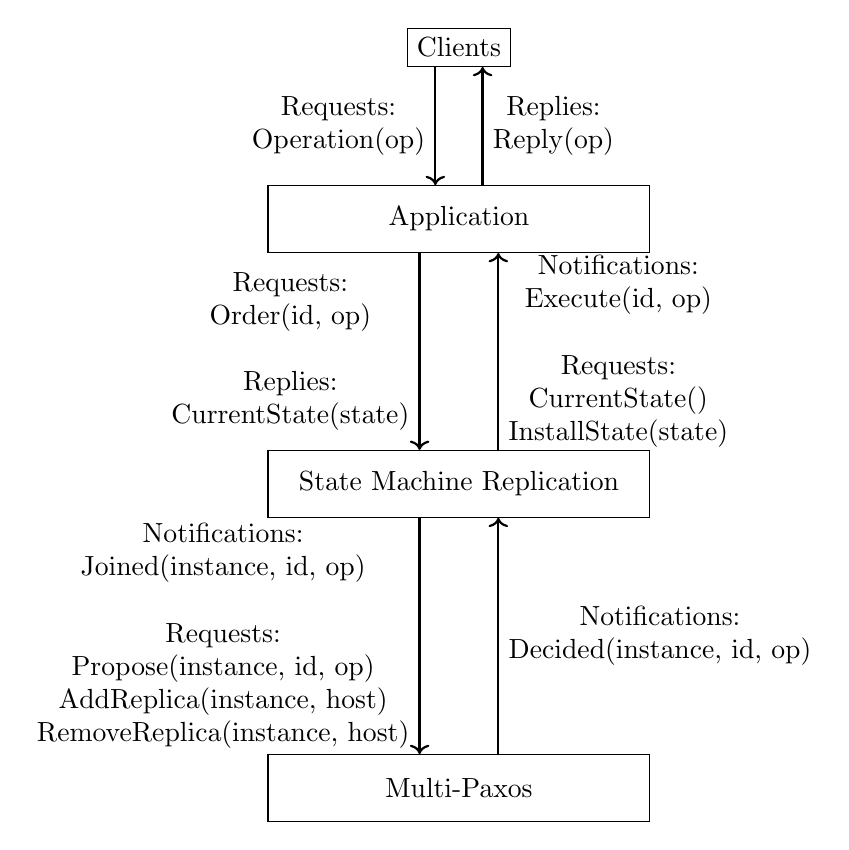
\begin{tikzpicture}[]  
    \node (clients) [draw, rectangle, minimum width=0.1\textwidth, minimum height=0.04\textwidth] {Clients};
    \node (app) [draw, rectangle, below=1.5 of clients, minimum width=0.4\textwidth, minimum height=0.07\textwidth] {Application};
    \node (smr) [draw, rectangle, below=2.5 of app, minimum width=0.4\textwidth, minimum height=0.07\textwidth] {State Machine Replication};
    \node (paxos) [draw, rectangle, below=3 of smr, minimum width=0.4\textwidth, minimum height=0.07\textwidth] {Multi-Paxos};

    \draw[->, thick] (clients.south) ++(-0.3, 0) -- ++(0,-1.5) node[midway, left, align=center] {Requests: \\ Operation(op)};
    \draw[<-, thick] (clients.south) ++(0.3,0) -- ++(0,-1.5) node[midway, right, align=center] {Replies: \\ Reply(op)};

    \draw[->, thick] (app.south) ++(-0.5, 0) -- ++(0,-2.5) node[midway, left, align=center] {Requests: \\ Order(id, op) \\  \\ Replies: \\ CurrentState(state)};
    \draw[<-, thick] (app.south) ++(0.5,0) -- ++(0,-2.5) node[midway, right, align=center] 
    {Notifications: \\ Execute(id, op) \\ \\ Requests: \\ CurrentState() \\ InstallState(state)};

    \draw[->, thick] (smr.south) ++(-0.5, 0) -- ++(0,-3) node[midway, left, align=center] {Notifications: \\ Joined(instance, id, op) \\ \\ Requests: \\ Propose(instance, id, op) \\ AddReplica(instance, host) \\ RemoveReplica(instance, host)};
    \draw[<-, thick] (smr.south) ++(0.5,0) -- ++(0,-3) node[midway, right, align=center] 
    {Notifications: \\ Decided(instance, id, op)};
\end{tikzpicture} \\

State Transfer: When a new replica joins the system, it must synchronize with the current state of the system. This process, known as state transfer, is managed by the SMR protocol. The protocol requests the current application state from the application and, upon receiving it, transmits this state along with information about the current sequence position to the new replica. To optimize this process, instead of involving all replicas, the replica that received the join request can respond to the new replica with the necessary state information. This requires the SMR protocol to exchange messages with other processes over the network. \\

Independence from the Agreement Protocol below: The implementation of the SMR protocol is independent of the underlying agreement protocol, with a few exceptions. For instance, when using Multi-Paxos, the SMR protocol must be informed about the current leader since only the leader proposes commands. In such cases, client requests received by non-leader replicas must be forwarded to the leader. If the leader changes, any unprocessed requests must be resubmitted to the new leader. Conversely, when using ABD, each instance of the protocol may require the SMR protocol to provide the system membership information for that instance. \\

Multi-Paxos Agreement Protocol: The Multi-Paxos agreement protocol determines the order of operations to be executed in the system. This protocol does not run multiple instances concurrently, due to the complexity of ensuring correctness, instead, every call from the State Machine is done one at-a-time. In accordance to the Multi-Paxos specification, only the leader proposes commands for agreement. Other replicas forward client requests to the leader, and participate in instances as instructed by the leader’s proposals. If a leader change occurs, pending client requests must be resubmitted to the new leader for ordering.

Careful management of system membership is critical in Multi-Paxos. Replicas must maintain an up-to-date view of the system membership to compute majorities accurately. Furthermore, a replica does not participate in instances from which it is excluded, either before joining the system, or after being removed from it. By adhering to these rules, the Multi-Paxos protocol ensures consistent and reliable agreement on the sequence of operations. \\

\section{Pseudo-code}

The following sub-sections describe in detail the pseudo-code for the provided Application Layer, and, most importantly, our concrete implementations for the ABD Quorum, State Machine, Multi-Paxos (Classic), and Multi-Paxos (Distinguished Learner) algorithms.

\subsection{Application}

The top-level Application is relatively trivial, as it's simply responsible for direct request and response handling between a client and an abstracted interface of the implemented DLT protocol, in the following flow: Client -> App -> DLT -> App -> Client. \\
The Application can handle concurrent requests from clients, managing them via the data and clientIdMapper Maps, which await responses from the underlying DLT layer. \\
Some separate request and notification handlers are implemented purely for the ABD protocol, given that operations are not yet abstracted via the SMR protocol, these handlers are: WriteComplete, ReadComplete, and UpdateValue. \\ 
To aid in understanding the implementation of this protocol, we present the pseudocode for this layer in the following block: \\

\begin{algorithmic}[1]
\small

\State \textbf{Interface:}
\State \quad Requests:
\State \quad \quad Operation(op, host)
\State \quad \quad CurrentState()
\State \quad \quad InstallState(state)
\State \quad \quad Execute(opId, op)
\State \quad Indications:
\State \quad \quad CurrentState(state)
\State \quad \quad Read(opId, opKey)
\State \quad \quad Write(opId, opKey, opData)\\

\State \textbf{State:}
\State \quad executedOps \Comment{Index for the most recently executed operation}
\State \quad data \Comment{Map (ID -> data) for storing data sent in requests}
\State \quad cumulativeHash
\State \quad clientIdMapper \Comment{Map (opID -> (cID, op)) containing client operations}
\State \quad strategy \Comment{Currently enabled replication strategy (ABD or SMR)} \\

\State \textbf{Upon Init(s) do:}
\State \quad executedOps $\gets$ 0
\State \quad data $\gets$ \{\}
\State \quad clientIdMapper $\gets$ \{\}
\State \quad cumulativeHash $\gets$ \{\}
\State \quad strategy $\gets$ s \\

\State \textbf{Upon CurrentState() do:}
\State \quad state $\gets$ (executedOps, cumulativeHash, data)
\State \quad \textbf{Trigger} CurrentState(state) \\

\State \textbf{Upon InstallState(state) do:}
\State \quad \textbf{Call} InstallStateProcedure(state) \\

\State \textbf{Upon Operation(op, host) do:}
\State \quad opUUID $\gets$ generateUUID()
\State \quad clientIdMapper[opId] $\gets$ {(host, op.opId,)}
\State \quad \textbf{if} (strategy = SMR) \textbf{then}
\State \quad \quad \textbf{Trigger} Order(opUUID, op.opType, op.key, op.data)
\State \quad \textbf{else}
\State \quad \quad \textbf{if} (op.opType = READ) \textbf{then}
\State \quad \quad \quad \textbf{Trigger Read}(opUUID, op.key)
\State \quad \quad \textbf{else}
\State \quad \quad \quad \textbf{Trigger Write}(opUUID, op.key, op.data) \\

\State \textbf{Upon Execute(opId, op) do:}
\State \quad cumulativeHash $\gets$ cumulativeHash $\cup$ {op.data}
\State \quad \textbf{if} (op.type = WRITE) \textbf{then}
\State \quad \quad data[op.key] $\gets$ op.data 
\State \quad executedOps $\gets$ executedOps + 1
\State \quad (client, opId) $\gets$ clientIdMapper[opId]
\State \quad clientIdMapper $\gets$ clientIdMapper \ {opId}
\State \quad \textbf{if} ((client, opId) = $\bot$) \textbf{then}
\State \quad \quad \textbf{return}
\State \quad \textbf{if} (op.type = WRITE) \textbf{then}
\State \quad \quad \textbf{Trigger Send}(REPLY, (opId, $\bot$), client)
\State \quad \textbf{else}
\State \quad \quad \textbf{Trigger Send}(REPLY, (opId, op.data), client) \\

\State \textbf{Upon WriteComplete(k, v, opId) do:}
\State \quad data[k] $\gets$ v
\State \quad (client, opId) $\gets$ clientIdMapper[opId]
\State \quad clientIdMapper $\gets$ clientIdMapper \ opId
\State \quad \textbf{Trigger Send}(REPLY, (opId, $\bot$), client)
\State \quad \textbf{Call} UpdateOperationCount() \\

\State \textbf{Upon ReadComplete(k, v, opId) do:}
\State \quad data[k] $\gets$ v
\State \quad (client, opId) $\gets$ clientIdMapper[opId]
\State \quad clientIdMapper $\gets$ clientIdMapper \ opId
\State \quad \textbf{Trigger} Send(REPLY, (opId, v), client)
\State \quad \textbf{Call} UpdateOperationCount() \\

\State \textbf{Upon UpdateValue(k, v) do:}
\State \quad data[k] $\gets$ v
\State \quad \textbf{Call} UpdateOperationCount() \\

\State \textbf{Upon UpdateOperationCount() do:}
\State \quad executedOps $\gets$ executedOps + 1
\State \quad \textbf{if} (executedOps \% 10000 = 0) \textbf{then}
\State \quad \quad cumulativeHash $\gets$ ComputeDataHash() \Comment{Computes hash of all keys currently stored in data Map}

\end{algorithmic} 

\subsection{ABD Quorum}

\subsubsection{Initialization}

The ABD Quorum protocol, although straightforward, also maintains a decent amount of state.

Starting off, each node needs to maintain its own unique ID, as well as the membership of all active nodes currently in the system, in order to send quorum messsages, and check if the number of replies surpasses the majority threshold.

Next up, the protocol maintains the index for the most up-to-date executed operation, which serves two main purposes: discarding messages from older operations, and storing/sending Tags for a given operation/quorum.

Naturally, we also store a set of quorum replies for the current operation, which basically consist of (Tag, opValue) pairs, in order to obtain the most recent value at the end of a quorum.

For every operation, a map of opKey -> Tags is also used, in order to store the most recent Tag for a given operation, alongside a map of opKey -> opValues, and, a map of opKey -> OpId (opKey-opValue pairs are the actual operation, at the application level, while opId is merely an identifier for an operation between the App and ABD layers).

Finally, pending merely stores a write value pending the completion of the current majority quorum, and is discarded after the write completes. \\

\begin{algorithmic}[1]
\small
\State \textbf{Interface:}
\State \quad Requests:
\State \quad \quad CurrentState(state)
\State \quad \quad Read(opId, opKey)
\State \quad \quad Write(opId, opKey, opData)
\State \quad Indications:
\State \quad \quad CurrentState()
\State \quad \quad InstallState(state)
\State \quad \quad Execute(opId, op)\\

\State \textbf{State:}
\State \quad thisHost \Comment{This node's host information}
\State \quad thisProcessId \Comment{This node's ID}
\State \quad membership \Comment{Set of node's currently in membership}
\State \quad opSeq \Comment{Current operation index}
\State \quad quorumReplies \Comment{Set of quorum replies regarding current operation}
\State \quad tags \Comment{Map of key -> (opSeq, processId)}
\State \quad values \Comment{Map of key -> opData}
\State \quad operations \Comment{Map of key -> opID}
\State \quad pending \Comment{Operation data pending to be written in current opSeq} \\

\State \textbf{Upon Init(h, initialMembership)} do:
\State \quad thisHost $\gets$ h
\State \quad membership $\gets$ initialMembership
\State \quad thisProcessId $\gets$ membership.indexOf(h)
\State \quad opSeq $\gets$ 0
\State \quad quorumReplies $\gets$ \{\}
\State \quad tags $\gets$ \{\}
\State \quad values $\gets$ \{\}
\State \quad operations $\gets$ \{\}
\State \quad pending $\gets$ $\bot$

\end{algorithmic}

\subsubsection{Read Operations}

Concerning read operations - the process is extremely streamlined: after the protocol receives a Read request from the App, it increments the current opSequence index, empties the quorumReplies set, and sets pending to null (given that it's a read operation, no value is pending to be written - this dynamic is subsequently used to facilitate some logic). 

Furthermore, the opKey mappings are added to both the operations and tags maps, in order to use them for comparisons with quorum replies. Finally, the Read request handler terminates by sending a QUORUM\_MSG to each peer in the membership. This message includes a $\top$ flag, signifying that it's a read operation, which enabled us to streamline both read and writes into one message handler. \\

Subsequently, peers then receive the QUORUM\_MSG via the QuorumMsg handler, which takes care of fetching the local Tag for the opKey in the current message, and, seeing as the operation is a read, the execution goes into the if branch, also fetches the local value for the opKey, and sends both the local Tag and value inside the READ\_REPLY to the original quorum sender. \\

Finally, the original quorum sender receives the aforementioned read replies via the ReadReplyMsg handler - which certifies that the message's opSequence is valid/current. Assuming it is, it checks if the pending value is null (which, as mentioned above, is used to facilitate some logic, including the reuse of quorumReplies for the next message's ACK's), and, if it is, adds the message to quorumReplies.

Once quorumReplies reaches the majority threshold, the maximum Tag is fetched from the set, pending is set to the value associated to the max Tag, opSeq is incremented, quorum replies emptied, and a WRITE\_MSG is sent to all peers, starting a new quorum with the purpose of keeping every node with the most up-to-date value.  \\

\begin{algorithmic}[1]
\small

\State \textbf{Upon Read(opId, opKey) do:}
\State \quad opSeq $\gets$ opSeq + 1
\State \quad quorumReplies $\gets$ \{\}
\State \quad pending $\gets$ $\bot$
\State \quad operations[opKey] $\gets$ {(opId)}
\State \quad tags[opKey] $\gets$ \{(opSeq, thisProcessId)\}
\State \quad \textbf{foreach} h $\in$ membership \textbf{do}
\State \quad \quad \textbf{Trigger Send}(QUORUM\_MSG, (opSeq, opKey, $\top$), h) \\

\State \textbf{Upon QuorumMsg((opSeq, opKey, isRead), h) do:}
\State \quad tag $\gets$ tags[opKey]
\State \quad \textbf{if} (isRead = $\top$) \textbf{then}
\State \quad \quad value $\gets$ values[opKey]
\State \quad \quad \textbf{Trigger Send}(READ\_REPLY\_MSG, (opSeq, tag, opKey, value), h)
\State \quad \textbf{else}
\State \quad \quad \textbf{Trigger Send}(READ\_TAG\_REPLY\_MSG, (opSeq, tag, opKey), h) \\

\State \textbf{Upon ReadReplyMsg((opSeq, tag, opKey, opValue), h)} do:
\State \quad \textbf{if} (this.opSeq $\neq$ opSeq) \textbf{then}
\State \quad \quad \textbf{return}
\State \quad \textbf{if} (pending = $\bot$) \textbf{then}
\State \quad \quad quorumReplies $\gets$ quorumReplies $\cup$ \{(tag, opValue)\}
\State \quad \textbf{if} (\#quorumReplies = (\#membership / 2) + 1) \textbf{then}
\State \quad \quad maxTagQuorumReply $\gets$ MaxTagQuorumReply(quorumReplies)
\State \quad \quad maxTag $\gets$ maxTagQuorumReply.tag
\State \quad \quad pending $\gets$ maxTagQuorumReply.opValue
\State \quad \quad opSeq $\gets$ opSeq + 1
\State \quad \quad quorumReplies $\gets$ \{\} 
\State \quad \quad \textbf{foreach} h $\in$ membership \textbf{do}
\State \quad \quad \quad \textbf{Trigger Send}(WRITE\_MSG, (opSeq, opKey, maxTag, pending), h) \\

\end{algorithmic}

\subsubsection{Write Operations}

Upon a write operation from the application, the Write handler is almost 1-to-1 compared to Read - it increments opSeq, empties quorumReplies, but - now pending is used to store the opData (whereas it was set to null on reads). Subsequently, the operations and tags mappings are exactly the same as on reads, and, the QUORUM\_MSG's are sent with a $\bot$ isRead flag. \\

Then, as mentioned previously, we reuse the QUORUM\_MSG (and consequently \textbf{QuorumMsg} handler, on the peer's end, by simply using a boolean flag \textbf{isRead} to distinguish read and write quorums), which implies that the QuorumMsg handler goes into the else branch, sending a READ\_TAG\_REPLY\_MSG with just the local Tag for the corresponding opKey. \\

This message is then handled by ReadTagReplyMsg, which, similarly to ReadReplyMsg, checks the validity of the message's opSeq, but, then checks if pending $\neq$ $\bot$, basically checking if the majority quorum is still to be reached, and, if so, adds the quorum reply. \\
Eventually, the majority is reached, and the max Tag quorum reply is fetched (which, in this case is only used to derive the max Tag opSequence number), opSeq is incremented, quorumReplies emptied in preparation for ACK messages, and, a new Tag is created with the most recent opSequence number (higher than the max Tag), which basically means that all nodes will be updated with the current write value. \\ And, as anticipated, a WRITE\_MSG is sent to every peer in a new quorum - setting pending to null, seeing as the write propagation is complete. \\

The other replicas then receive this write via the WriteMsg handler (which is used at the end of reads as mentioned prior), and, if the message's Tag for the corresponding opKey is superior to the local Tag for the same opKey (which, for original write operations, it's guaranteed to be, but, for originally read operations, it might not be), the tag and value relating to the opKey is replaced with the message's contents. \\
Subsequently, if the message came from another peer, the UpdateValue notification to the App layer is triggered. Then, an ACK\_MSG is sent back to the original sender of the write quorum. \\

Upon receiving the ACK\_MSG via the final AckMsg handler, it checks if the opSequence number is valid, adds the quorum reply to quorumReplies, and, when it reaches a majority, it empties the quorumReplies set, and verifies if pending = $\bot$, which, by the logic explained prior, means the operation was originally a Write, or, a Read - triggering the corresponding operation completion to the Application layer. \\

\begin{algorithmic}[1]
\small

\State \textbf{Upon Write(opId, opKey, opData) do}:
\State \quad opSeq $\gets$ opSeq + 1
\State \quad quorumReplies $\gets$ \{\}
\State \quad pending $\gets$ opData
\State \quad operations[opKey] $\gets$ {(opId)}
\State \quad tags[opKey] $\gets$ \{(opSeq, thisProcessId)\}
\State \quad \textbf{foreach} h $\in$ membership \textbf{do}
\State \quad \quad \textbf{Trigger Send}(QUORUM\_MSG, (opSeq, opKey, $\bot$), h) \\

\State \textbf{Upon ReadTagReplyMsg((opSeq, tag, opKey), h) do:}
\State \quad \textbf{if} (this.opSeq $\neq$ opSeq) \textbf{then}
\State \quad \quad \textbf{return}
\State \quad \textbf{if} (pending $\neq$ $\bot$) \textbf{then}
\State \quad \quad quorumReplies $\gets$ quorumReplies $\cup$ \{(tag, $\bot$)\}
\State \quad \textbf{if} (\#quorumReplies = (\#membership / 2) + 1) \textbf{then}
\State \quad \quad maxTagOpSeq $\gets$ MaxTagQuorumReply(quorumReplies).tag.opSeq
\State \quad \quad opSeq $\gets$ opSeq + 1
\State \quad \quad quorumReplies $\gets$ \{\} 
\State \quad \quad newTag $\gets$ (maxTagOpSeq + 1, thisProcessId) 
\State \quad \quad \textbf{foreach} h $\in$ membership \textbf{do}
\State \quad \quad \quad \textbf{Trigger Send}(WRITE\_MSG, (opSeq, opKey, newTag, pending), h)
\State \quad \quad pending $\gets$ $\bot$ \\

\State \textbf{Upon WriteMsg((opSeq, tag, opKey, opValue), h) do:}
\State \quad thisTag $\gets$ tags[opKey]
\State \quad \textbf{if} (tag > thisTag) \textbf{then}
\State \quad \quad tags[opKey] $\gets$ tag
\State \quad \quad values[opKey] $\gets$ opValue
\State \quad \quad \textbf{if} (h $\neq$ thisHost) \textbf{then}
\State \quad \quad \quad \textbf{Trigger UpdateValue}(opSeq, opKey, opValue) 
\State \quad \textbf{Trigger Send}(ACK\_MSG, (opSeq, opKey), h)  \\

\State \textbf{Upon AckMsg((opSeq, opKey), h) do:}
\State \quad \textbf{if} (this.opSeq $\neq$ opSeq) \textbf{then}
\State \quad \quad \textbf{return}
\State \quad quorumReplies $\gets$ quorumReplies $\cup$ \{((opSeq, thisProcessId), pending)\}
\State \quad \textbf{if} (\#quorumReplies $\neq$ (\#membership / 2) + 1) \textbf{then}
\State \quad \quad \textbf{return}
\State \quad quorumReplies $\gets$ \{\}
\State \quad \textbf{if} (pending = $\bot$) \textbf{then}
\State \quad \quad \textbf{Trigger WriteComplete}(opSeq, opKey, values[opKey], operations[opKey])
\State \quad \textbf{else}
\State \quad \quad \textbf{Trigger ReadComplete}(opSeq, opKey, pending, operations[opKey]) \\
\end{algorithmic} \\

\subsection{State Machine}
\subsubsection{Initialization}
There are two ways to join our system: either through the initial membership or by contacting a replica that is already part of the system. In our configuration, a replica that is not part of the system will request to join the system by contacting the first position of the initialMembership it receives as a parameter. The new replica will also have a timer, as it acts as a client during this process. If it is not added within a certain period, it will retry the connection. More details about this process will be elaborated in the AddReplica section of the state machine protocol.

On the other hand, during initialization, if a replica is part of the initialMembership, it will join the system immediately. The process with the highest processId (in our configuration, the process with the highest index in the initial membership list) will attempt to become the leader. As a result, even before receiving the first order from the HashApp, our system will already have a leader to propose requests to our agreement layer, which can be either the distinguished or Classic variant of Paxos.

\subsubsection{Initialization and OrderRequest PseudoCode}
\begin{algorithmic}[1]
\small
\State \textbf{Interface:}
\State \quad Requests:
\State \quad \quad CurrentState(state)
\State \quad \quad Read(opId, opKey)
\State \quad \quad Write(opId, opKey, opData)
\State \quad Indications:
\State \quad \quad CurrentState()
\State \quad \quad InstallState(state)
\State \quad \quad Execute(opId, op)\\

\State \textbf{State:}
\State \quad thisHost \Comment{This node's host information}
\State \quad state \Comment{JOINING or ACTIVE}
\State \quad membership \Comment{Set of node's currently in membership}
\State \quad nextInstance \Comment{Current operation index}
\State \quad leader \Comment{Leader node's host information}
\State \quad previousLeader \Comment{Previous leader Candidate}
\State \quad replcaIdSet \Comment{Hosts that contacted this replica to join}
\State \quad pendingOrders \Comment{Pending Orders to be executed by leader}
\State \quad pendingAddRemoves \Comment{Pending addRemove operations to be executed by leader, value pair of (host, boolean). True = Add ; False = Remove}
\State \quad executedOperations \Comment{Orders to be executed by at the SMR Layer}
\State \quad executedAddRemoves \Comment{Add/Remove operations executed at the SMR Layer} 
\State \quad hostTimers \Comment{(timerId, Host) to know the which Hosts timer triggered}
\State \quad hostRetries \Comment{(Host, retriesNr) how many more connection retries for given Host}
\\


\State \textbf{Upon Init(h, initialMembership)} do:
\State \quad thisHost $\gets$ h
\State \quad nextInstance $\gets$ 1
\State \quad leader $\gets$ $\bot$
\State \quad contact $\gets$ $\bot$
\State \quad replicaIdSet $\gets$ \{\}
\State \quad pendingOrders $\gets$ \{\}
\State \quad pendingAddRemoves $\gets$ \{\}
\State \quad executedOperations $\gets$ \{\}
\State \quad executedAddRemoves $\gets$ \{\}
\State \quad hostTimers $\gets$ \{\}
\State \quad hostRetries $\gets$ \{\}

\State \quad \textbf{if} (thisHost $\in$ initialMembership) \textbf{then}
\State \quad \quad state $\gets$ ACTIVE
\State \quad \quad membership $\gets$ initialMembership
\State \quad \quad \textbf{Trigger Joined}(membership, membership.indexOf(thisHost), $\top$)
\State \quad \quad firstLeader $\gets$ membership[\#membership - 1]
\State \quad \quad \textbf{if} (firstLeader = thisHost) \textbf{then}
\State \quad \quad \quad \textbf{Trigger Prepare}(nextInstance)
\State \quad \textbf{else} 
\State \quad \quad state $\gets$ JOINING
\State \quad \quad membership $\gets$ initialMembership
\State \quad \quad membership $\gets$ membership $\cup$ \{(thisHost)\}
\State \quad \quad \textbf{Trigger Send}(ADD\_REPLICA, (thisHost, 0, initialMembership[0]), initialMembership[0])
\State \quad \quad \textbf{Setup Timer (AddReplicaTimer, 3)} \\

\State \textbf{Upon Order(opId, opKey, opData) do}:
\State \quad \textbf{if} (state = JOINING) \textbf{then}
\State \quad \quad pendingOrders $\gets$ pendingOrders $\cup$ \{(opId, ipData)\}
\State \quad \quad \textbf{return}
\State \quad \textbf{if} (leader = $\bot$) \textbf{then}
\State \quad \quad pendingOrders $\gets$ pendingOrders $\cup$ \{(opId, ipData)\}
\State \quad \textbf{else if} (thisHost = leader) \textbf{then}
\State \quad \quad \textbf{Trigger Propose}(nextInstance, opId, opData)
\State \quad \quad nextInstance $\gets$ nextInstance + 1
\State \quad \textbf{else}
\State \quad \quad pendingOrders[opId] $\gets$ \{(opData)\}
\State \quad \quad \textbf{Trigger Send}(LEADER\_ORDER\_MSG, (nextInstance, opId, opData), leader) \\

\State \textbf{Upon Decided(instance, opId, op) do}:
\State \quad \textbf{if} (thisHost $\neq$ leader) \textbf{then}
\State \quad \quad nextInstance $\gets$ nextInstance + 1
\State \quad pendingOrders $\gets$ pendingOrders $\setminus$ \{(opId) \}
\State \quad executedOperations $\gets$ executedOperations $\cup$ \{(opId, op)\}
\State \quad \textbf{Trigger Execute}(opId, op) \\

\end{algorithmic}

\subsubsection{Order Request}
In MultiPaxos, only the leader is responsible for proposing requests. Therefore, when a replica receives a request from its App Layer, it will forward the request to the leader if it is not the leader itself. If the replica is in the process of joining, the request will be buffered and held until the replica has fully joined the system, at which point it will be forwarded to the leader. Similarly, if no leader has been elected, requests are buffered and stored until a leader is chosen. Once a leader is in place, these pending requests are forwarded to the leader for processing. This mechanism ensures that requests are not lost and are eventually handled once a leader is available. \\

\subsubsection{Decision}
Once the Agreement Layer reaches consensus on an operation, it triggers the Decided Notification, which increments the state machine operation instance—except for the leader, whose instance is incremented when they propose the operation. The notification removes the operation from pendingOperations (if present) and places the decided operation in executedOperations. Finally, it propagates the operation to the Hash App Layer, which is responsible for maintaining the overall application state. \\

\subsubsection{Add/Remove Replica}
As mentioned in the initialization section, when a replica wants to join the system, it will contact an existing replica within the system. If the contacted replica is not the leader, it will forward the operation to the leader so that the leader can propose the AddReplica request. Once consensus is reached, each replica will add the new replica to their membership. The contacted replica, which will now the new replica in its replicaIdMapper upon contact, will request its own HashApp for the current state. This request will include the instance in which the new replica joined the system.

\subsubsection{Add/Remove Replica PseudoCode}
\begin{algorithmic}[1]
\small
\State \textbf{Upon AddReplica(newReplica, contact, instance) do}:
\State \quad \textbf{if} (leader = $\bot$ $\lor$ (replica $\in$ pendingAddRemoves)) \textbf{then}
\State \quad \quad \textbf{return}
\State \quad \textbf{if} (thisHost = contact) \textbf{then}
\State \quad \quad replicaIdSet $\gets$ replicaIdSet $\cup$ \{newReplica\}
\State \quad \textbf{foreach} $((k, v) \in \text{executedAddRemoves})$ \textbf{do}
\State \quad \quad \textbf{if} $(v.\text{getLeft}() = \text{newReplica} \land v.\text{getRight}() = \top)$ \textbf{then}
\State \quad \quad \quad \textbf{TriggerCurrentState}(\text{instance})
\State \quad \quad \quad \textbf{return}
\State \quad \textbf{if} (thisHost $\neq$ leader) \textbf{then}
\State \quad \quad \textbf{Trigger Send}(ADD\_REPLICA\_MSG, (newReplica, nextInstance, contact), leader)
\State \quad \quad \textbf{return}
\State \quad \textbf{Trigger Connect}(newReplica)
\State \quad nextInstance $\gets$ nextInstance + 1
\State \quad \textbf{Trigger AddReplica}(nextInstance, newReplica) \\

\State \textbf{Upon MembershipChange(isAdding, replica, instance) do}:
\State \quad \textbf{if} (isAdding = $\top$) \textbf{then}
\State \quad \quad \quad \textbf{Trigger Connect}(replica)
\State \quad \quad \quad membership $\gets$ membership $\cup$ \{replica\}

\State \quad \quad \textbf{if} (replica $\in$ replicaIdSet) \textbf{then}
\State \quad \quad \quad replicaIdSet $\gets$ replicaIdSet $\setminus$ \{(replica)\}
\State \quad \quad \quad \textbf{Trigger CurrentState}(instance)
\State \quad \textbf{else}
\State \quad \quad \textbf{Trigger CloseConnection}(replica)
\State \quad \quad membership $\gets$ membership $\setminus$ \{(replica)\}
\State \quad \textbf{if} (thisHost $\neq$ leader) \textbf{then}
\State \quad \quad nextInstance $\gets$ nextInstance + 1 \\

\State \textbf{Upon CurrentState(instance, state) do}:
\State \quad \textbf{if} (leader = $\bot$) \textbf{then}
\State \quad \quad \textbf{return}
\State \quad newReplica $\gets$ executedAddRemoves[instance].host
\State \quad \textbf{Trigger Send}(REPLICA\_ADDED\_MSG, (instance, state, membership, leader), newReplica) \\

\State \textbf{Upon ReplicaAdded(newState, instance, newMembership, l) do}:
\State \quad leader $\gets$ l
\State \quad nextInstance $\gets$ instance
\State \quad membership $\gets$ newMembership
\State \quad \textbf{foreach} m $\in$ membership \textbf{do}
\State \quad \quad \textbf{Trigger Connect}(m)
\State \quad \textbf{Trigger InstallState}(newState)
\State \quad \textbf{Trigger Joined}(membership, nextInstance, leader)
\State \quad state $\gets$ ACTIVE
\State \quad \textbf{foreach} (orderId, value) $\in$ pendingOrders \textbf{do}
\State \quad \quad \textbf{Trigger Send}(LEADER\_ORDER\_MSG, (0, orderId, value), leader) \\

\State \textbf{Upon Timer AddReplicaTimer() do:}
\State \quad \textbf{if} (state = State.ACTIVE) \textbf{then}
\State \quad \quad \textbf{return}
\State \quad \textbf{if} (membership.\text{size}() = 0) \textbf{then}
\State \quad \quad \textbf{Terminate Program}
\State \quad contact $\gets$ membership.\text{get}(0)
\State \quad \textbf{if} (state = \text{State.JOINING}) \textbf{then}
\State \quad \quad membership.\text{remove}(node)
\State \quad \textbf{else if} (leader = \text{null}) \textbf{then}
\State \quad \quad pendingAddRemoves.\text{put}(node, \text{false})
\State \quad \textbf{else if} (self.\text{equals}(leader)) \textbf{then}
\State \quad \quad \textbf{Trigger RemoveReplica}(nextInstance $\gets$ nextInstance + 1, node) \\
\end{algorithmic}

Upon receiving the state in reply, the contacted replica will send the state to the new replica, along with the identity of the leader, the updated membership of the system, and the instance in which the new replica joined (as returned by the current state request). This joinedInstance is essential for the new replica to "catch up" to the current state of the leader. The new replica can do so either by making a Log Request to the leader with the snapshot of the system (Classic Paxos) or by receiving the undecided messages in the Paxos layer before joining(Distinguished Learner Paxos). Once the new replica has installed the state it received, it will transition from JOINING to ACTIVE and become ready to process requests from its HashApp layer. Additionally, it will flush any orders accumulated during the JOINING state at the state machine protocol level, trigger the JoinedNotification in the agreement layer, and fully catch up to the log state.

In addition to this, several fault tolerance mechanisms have been implemented to make the addition process more robust. Firstly, there is the AddReplicaTimer. If the new replica does not contact the designated replica or if the message fails to reach the leader (either due to failure of the contact replica or because the leader is down), the timer will simply retry the operation. Additionally, whenever a replica within the membership of the new replica fails, it will be removed from the membership. This mechanism rotates the contacts for the new replica and ensures termination. Specifically, if there are no remaining members in the membership of the new replica, the process will terminate, and all other replicas will initiate a RemoveReplica request if the AddReplica operation had received a majority but was not completed.

If the AddReplica operation has already been initiated, but is still pending (not yet decided), the timer will simply retry the operation. However, if the operation is already present in the executed messages, it means that the decision was made previously, but the new replica was not informed by the previous contact when the decision occurred. In this case, the contacted replica will immediately initiate the state transfer to the new replica. This ensures that the operation is not repeated unnecessarily. To further prevent duplication, the new replica will reject any state transfer if it does not come from its most recent contact, ensuring that the state is only accepted once and from the correct source.

A replica is removed when the membership detects it has failed, either by being unable to establish a connection or by an ongoing connection failing. In the case of a failed connection attempt, after a certain number of retries, the leader will propose a request to remove the failed replica. If no leader exists, the request is buffered in a list and will be processed once a new leader is elected. The process is similar when an established connection goes down, with the key difference that a new leader may be re-elected, as other replicas in the membership will detect the failure of their connection to any replica, including leader.

\subsubsection{Connection Failures and Leader Election PseudoCode}
\begin{algorithmic}[1]
\small
\State \textbf{Upon LeaderMsgFail(opId, op, instance, host) do}:
\State \quad \textbf{if} (leader = $\bot$) \textbf{then}
\State \quad \quad pendingOrders[opId] $\gets$ op
\State \quad \textbf{else}
\State \quad \quad \textbf{Send}(LEADER\_ORDER\_MSG, (opId, op, instance), host) \\

\State \textbf{Upon OutConnectionDown(host) do}:
\State \quad \textbf{if} (leader = $\bot$ or host = leader) \textbf{then}
\State \quad \quad pendingAddRemoves[host] $\gets$ $\bot$
\State \quad \textbf{if} (host = leader) \textbf{then}
\State \quad \quad previousLeader $\gets$ leader
\State \quad \quad leader $\gets$ $\bot$
\State \quad \quad \textbf{Call NextLeaderCandidate}
\State \quad \textbf{Trigger CloseConnection}(host)
\State \quad \textbf{if} (thisHost = leader) \textbf{then}
\State \quad \quad nextInstance $\gets$ nextInstance + 1 
\State \quad \quad \textbf{Trigger RemoveReplica}(nextInstance, node) \\

\State \textbf{Upon OutConnectionFailed(host) do}:
\State \quad tid = \textbf{Setup Timer ConnectionRetryTimer}(0.05)
\State \quad hostTimers $\gets$ hostTimers $\cup$ \{(tid, host)\}
\State \quad \textbf{if} (host $\notin$ hostRetries) \textbf{then}
\State \quad \quad hostRetries $\gets$ hostRetries $\cup$ \{(host, MAXRETRIES)\} \\

\State \textbf{Upon Timer ConnectionRetryTimer(t, tid) do:}
\State \quad node $\gets$ hostTimers.\text{remove}(tid)
\State \quad r $\gets$ hostRetries.\text{computeIfPresent}(node, \text{(key, value) $\rightarrow$ value - 1})
\State \quad \textbf{if} (r $\neq$ \text{null} \textbf{and} r $> 0$ \textbf{and} membership.\text{contains}(node)) \textbf{then}
\State \quad \quad \textbf{Trigger Connect}(node)
\State \quad \quad \textbf{return}
\State \quad hostRetries.\text{remove}(node)
\State \quad \textbf{if} (state = \text{State.JOINING}) \textbf{then}
\State \quad \quad membership.\text{remove}(node)
\State \quad \textbf{else if} (leader = \text{null}) \textbf{then}
\State \quad \quad pendingAddRemoves.\text{put}(node, \text{false})
\State \quad \textbf{else if} (self.\text{equals}(leader)) \textbf{then}
\State \quad \quad \textbf{Trigger RemoveReplica}(nextInstance $\gets$ nextInstance + 1, node) \\

\State \textbf{Procedure NextLeaderCandidate() do}:
\State \quad \textbf{foreach Descending} (h $\in$ membership) \textbf{then}
\State \quad \quad \textbf{if} (pendingAddRemoves[h] = $\bot$ or h $\neq$ previousLeader) \textbf{then}
\State \quad \quad \quad \textbf{if} (h = thisHost) \textbf{then}
\State \quad \quad \quad \quad previousLeader = h
\State \quad \quad \quad \quad \textbf{Trigger Prepare}(nextInstance)
\State \quad \quad \quad \textbf{else}
\State \quad \quad \quad \quad \textbf{break}
\State \quad \textbf{Setup Timer LeaderCandidateTimer}(1000) \\

\State \textbf{Upon Timer LeaderCandidateTimer(t, tid) do:}
\State \quad \textbf{if} (leader = $\bot$) \textbf{then}
\State \quad \quad \textbf{Call NextLeaderCandidate}
\State \quad \textbf{else}
\State \quad \quad previousLeader $\gets$ \text{null}

\end{algorithmic}

\subsubsection{Leader Election}
At the state machine protocol layer, once the failure of the leader is detected, a recursive process is initiated to select a new leader. This process begins by selecting a replica (starting from the highest index) that is neither the previous leader, nor one marked for removal, nor in the joining state. The candidate replica will then issue a prepare request to the agreement layer. All replicas must agree on the new leader, or the timer will trigger a retry.

Once the leader initiates the prepareRequest, and the agreement layer reaches consensus, the new leader will receive all accepted messages that occurred past its own accepted instance. This allows the new leader to reissue these messages in the same order they were commited to all replicas. Additionally, any messages that were waiting for a leader election to be completed will be issued by the new leader in an arbitrary order, including Add and Remove Replica operations

\subsubsection{New Leader and Leader Orders PseudoCode}
\begin{algorithmic}[1]
\small
\State \textbf{Upon NewLeader(newLeader, prepareOkMsgs) do}:
\State \quad leader $\gets$ newLeader
\State \quad \textbf{if} (thisHost $=$ leader) \textbf{then}
\State \quad \quad \textbf{foreach} (msg $\in$ prepareOkMsgs) \textbf{do}
\State \quad \quad \quad pendingOrders $\gets$ pendingOrders $\setminus$ \{(msg.id)\}
\State \quad \quad \quad nextInstance $\gets$ nextInstance + 1
\State \quad \quad \quad \textbf{Trigger Propose}(nextInstance, msg.id, msg.value)
\State \quad \quad \textbf{foreach} ((host, isPending) $\in$ pendingAddRemoves) \textbf{do}
\State \quad \quad \quad nextInstance $\gets$ nextInstance + 1
\State \quad \quad \quad \textbf{if} (isPending = $\top$) \textbf{then}
\State \quad \quad \quad \quad \textbf{Trigger AddReplica}(nextInstance, host)
\State \quad \quad \quad \textbf{else}
\State \quad \quad \quad \quad \textbf{Trigger RemoveReplica}(nextInstance, host)
\State \quad \quad \textbf{foreach} ((oId, value) $\in$ pendingOrders) \textbf{do}
\State \quad \quad \quad nextInstance $\gets$ nextInstance + 1
\State \quad \quad \quad \textbf{Trigger Propose}(nextInstance, oId, value)
\State \quad \textbf{else}
\State \quad \quad \textbf{foreach} (order $\in$ pendingOrders) \textbf{do}
\State \quad \quad \quad \textbf{Trigger Send}(LEADER\_ORDER\_MSG, (0, order.key, order.value), leader)
\State \quad pendingOrders $\gets$ \{\} 
\State \quad pendingAddRemoves $\gets$ \{\} \\

\State \textbf{Upon LeaderOrder(instance, opId, op) do}:
\State \quad \textbf{if} (leader = $\bot$) \textbf{then}
\State \quad \quad pendingOrders[opId] $\gets$ op
\State \quad \quad \textbf{return}
\State \quad nextInstance $\gets$ nextInstance + 1 
\State \quad \textbf{Trigger Propose}(nextInstance, opId, op) \\

\end{algorithmic}


\subsection{Multi-Paxos (Classic)}
\begin{algorithmic}[1]
\small
\State \textbf{Interface:}
\State \quad Requests:
\State \quad \quad Propose(instance, id, op)
\State \quad \quad AddReplica(instance, host)
\State \quad \quad RemoveReplica(instance, host)
\State \quad Indications:
\State \quad \quad Decided(instance, id, op)\\

\State \textbf{State:}
\State \quad thisHost \Comment{This node's host information}
\State \quad joinedInstance \Comment{This node's index in the membership}
\State \quad prepareOkCount \Comment{Number of PrepareOk messages received for the current operation}
\State \quad highestPrepare \Comment{Highest node index of received PrepareOk messages}
\State \quad membership \Comment{Set of node's currently in membership}
\State \quad toBeDecidedIndex \Comment{To be decided index}
\State \quad instanceStateMap \Comment{Map of each instance's: index -> (acceptOkCount, isDecided)}
\State \quad toBeDecidedMessages \Comment{Map of index -> (opId, opValue)}
\State \quad acceptedMessages \Comment{Map of index -> (opId, opValue)}
\State \quad addReplicaInstances \Comment{Map of index -> (host, isAdding)} \\

\State \textbf{Upon Init(h, initialMembership)} do:
\State \quad thisHost $\gets$ h
\State \quad joinedInstance $\gets$ -1
\State \quad membership $\gets$ $\bot$
\State \quad prepareOkCount $\gets$ 0
\State \quad highestPrepare $\gets$ 0
\State \quad toBeDecidedIndex $\gets$ 1
\State \quad toBeDecidedMessages $\gets$ \{\}
\State \quad acceptedMessages $\gets$ \{\}
\State \quad addReplicaInstances $\gets$ \{\}
\State \quad prepareOkMessages $\gets$ \{\}
\State \quad instanceStateMap $\gets$ \{\} \\

\State \textbf{Upon Prepare(instance) do}:
\State \quad prepareOkCount $\gets$ 0
\State \quad highestPrepare $\gets$ highestPrepare + 1
\State \quad \textbf{foreach} (h $\in$ membership) \textbf{do}
\State \quad \quad \textbf{Trigger Send}(PREPARE\_MSG, (highestPrepare, instance, $\bot$), h) \\

\State \textbf{Upon PrepareMsg((seqNumber, instance, isOk), h) do}:
\State \quad \textbf{if} (seqNumber < highestPrepare) \textbf{then}
\State \quad \quad \textbf{return}
\State \quad highestPrepare $\gets$ seqNumber
\State \quad relevantMessages $\gets$ \{\}
\State \quad \textbf{if} (thisHost $\neq$ h $\land$ \text{joinedInstance} $\geq$ 0) \textbf{then}
\State \quad \quad \textbf{foreach} (m $\in$ acceptedMessages) \textbf{do}
\State \quad \quad \quad \textbf{if} (m.\text{instance} $\geq$ instance) \textbf{then}
\State \quad \quad \quad \quad relevantMessages $\gets$ relevantMessages $\cup$ \{m\}
\State \quad \quad \textbf{Trigger NewLeader}(h)
\State \quad \quad toBeDecidedMessages $\gets$ \{\}
\State \quad \textbf{Trigger Send}(PREPARE\_OK\_MSG, (highestPrepare, relevantMessages), h) \\

\State \textbf{Upon PrepareOkMsg((seqNumber, relevantMessages), h) do}:
\State \quad \textbf{if} (seqNumber < highestPrepare) \textbf{then}
\State \quad \quad \textbf{return}
\State \quad prepareOkCount $\gets$ prepareOkCount + 1
\State \quad \textbf{if} (\#relevantMessages $> $ \#prepareOkMessages) \textbf{then}
\State \quad \quad prepareOkMessages $\gets$ relevantMessages
\State \quad \textbf{if} (prepareOkCount $\ge$ (\#membership / 2) + 1) \textbf{then}
\State \quad \quad prepareOkCount $\gets$ -1
\State \quad \quad \textbf{Trigger NewLeader}(thisHost, prepareOkMessages)
\State \quad \quad prepareOkMessages $\gets$ \{\} \\

\State \textbf{Upon Joined(jMembership, instance, leader) do}:
\State \quad membership $\gets$ jMembership
\State \quad toBeDecidedIndex $\gets$ joinedInstance 
\State \quad \textbf{if} (notification.\text{getContact}() $\neq$ \text{null} \textbf{and} toBeDecidedIndex $> 1$) \textbf{then}
\State \quad \quad\textbf{Trigger Send}(LOGREAD\_MSG, (toBeDecidedIndex), leader)
\State \quad \textbf{else}
\State \quad \quad joinedInstance $\gets$ toBeDecidedIndex \\

\State \textbf{Upon LogReadMsg((instance), h) do}:
\State \quad \text{accMsgs} $\gets$ \text{acceptedMessages}\( \text{.tailMap} [\text{msg.getInstance()}, \infty] \)
\State \quad \textbf{Trigger Send}(LOGWRITE\_MSG, $(t, hp, a, tbd, ri, \text{leader})$) \\

\State \textbf{Upon LogWriteMsg((m), h) do}:
\State \quad toBeDecidedIndex $\gets$ m.\text{getInstance}()
\State \quad joinedInstance $\gets$ toBeDecidedIndex
\State \quad highest\_prepare $\gets$ m.\text{getHighestPrepare}()
\State \quad acceptedMessages $\gets$ m.\text{getAcceptedMessages}()
\State \quad toBeDecidedMessages.\text{putAll}(m.\text{getToBeDecidedMessages}())
\State \quad addReplicaInstances $\gets$ m.\text{getAddReplicaInstances}()
\State \quad \textbf{for each} (k, v) \textbf{in} acceptedMessages \textbf{do}
\State \quad \quad \textbf{if} (addReplicaInstances.\text{containsKey}(k)) \textbf{then}
\State \quad \quad \quad r $\gets$ addReplicaInstances.\text{get}(k)
\State \quad \quad \quad \textbf{Trigger Send}(CHANGE\_MEMBERSHIP\_MSG, (k, r.\text{getLeft}(), r.\text{getRight}()))
\State \quad \quad \textbf{else}
\State \quad \quad \quad \textbf{Trigger Decided}(k, v.\text{getLeft}, v.\text{getRight}) \\

\State \textbf{Upon AddReplica(instance, host) do}:
\State \quad \textbf{foreach} (h $\in$ membership) \textbf{do}
\State \quad \quad \textbf{Trigger Send}(CHANGE\_MEMBERSHIP\_MSG, (host, instance, highestPrepare, $\bot$, $\top$), h) \\

\State \textbf{Upon RemoveReplica(instance, host) do}:
\State \quad \textbf{foreach} (h $\in$ membership) \textbf{do}
\State \quad \quad \textbf{if} (h $\neq$ host) \textbf{then}
\State \quad \quad \quad \textbf{Trigger Send}(CHANGE\_MEMBERSHIP\_MSG, (host, instance, highestPrepare, $\bot$, $\bot$), h) \\

\State \textbf{Upon Propose(instance, opId, op) do}:
\State \quad \textbf{foreach} (h $\in$ membership) \textbf{do}
\State \quad \quad \textbf{Trigger Send}(ACCEPT\_MSG, (instance, highestPrepare, opId, op), h) \\

\State \textbf{Upon ChangeMembershipMsg((host, instance, seqNumber, isAdding, isOk, mToBeDecidedMsgs, mAddReplicaInstances), h) do}:
\State \quad \textbf{if} (seqNumber < highestPrepare) \textbf{then}
\State \quad \quad \textbf{return}
\State \quad highestPrepare $\gets$ seqNumber
\State \quad \textbf{if} (isAdding = $\bot$) \textbf{then}
\State \quad \quad membership $\gets$ membership,remove(host)
\State \quad instanceStateMap[instance] $\gets$ (0, $\bot$)
\State \quad acceptOkMsg $\gets$ (instance, seqNumber, GenerateUUID(), {})
\State \quad toBeDecidedMessages[instance] $\gets$ (acceptOkMsg.opId, acceptOkMsg.op)
\State \quad addReplicaInstances[instance] $\gets$ (host, isAdding)
\State \quad \textbf{foreach} (h $\in$ membership) \textbf{do}
\State \quad \quad \textbf{Trigger Send}(ACCEPT\_OK\_MSG, acceptOkMsg, h) \\

\State \textbf{Upon AcceptMsg((opId, instance, op, seqNumber, lastChosen), h) do}:
\State \quad \textbf{if} (seqNumber < highestPrepare) \textbf{then}
\State \quad \quad \textbf{return}
\State \quad highestPrepare $\gets$ seqNumber
\State \quad toBeDecidedMessages[instance] $\gets$ (opId, op)
\State \quad \textbf{if} (joinedInstance $\ge$ 0) \textbf{then}
\State \quad \quad instanceStateMap[instance] $\gets$ (0, $\bot$)
\State \quad \quad \textbf{foreach} (h $\in$ membership) \textbf{do}
\State \quad \quad \quad \textbf{Trigger Send}(ACCEPT\_OK\_MSG, (opId, instance, op, seqNumber), h) \\

\State \textbf{Upon AcceptOkMsg((opId, instance, op, seqNumber), h) do}:
\State \quad \textbf{if} (instanceStateMap[instance] = $\bot$) \textbf{then}
\State \quad \quad \textbf{return}
\State \quad \textbf{if} (seqNumber = > highestPrepare) \textbf{then}
\State \quad \quad state.acceptOkCount $\gets$ 0
\State \quad state.acceptOkCount $\gets$ state.acceptOkCount + 1
\State \quad \textbf{if} (state.acceptOkCount $\ge$ (\#membership / 2) + 1 and state.isDecided = $\bot$) \textbf{then}
\State \quad \quad state.isDecided $\gets$ $\top$
\State \quad \quad \textbf{while} (toBeDecidedIndex $\le$ instance) \textbf{do}
\State \quad \quad \quad pair $\gets$ toBeDecidedMessages[toBeDecidedIndex]
\State \quad \quad \quad toBeDecidedMessages $\gets$ toBeDecidedMessages.remove(toBeDecidedIndex)
\State \quad \quad \quad \textbf{if} (pair $\neq$ $\bot$) \textbf{then}
\State \quad \quad \quad \quad \textbf{break}

\State \quad \quad \quad acceptedMessages[toBeDecidedIndex] $\gets$ pair
\State \quad \quad \quad \textbf{if} (addReplicaInstance[toBeDecidedIndex] $\neq$ $\bot$) \textbf{then}
\State \quad \quad \quad \quad \textbf{Trigger Decided}(toBeDecidedIndex, pair.opId, pair.op)
\State \quad \quad \quad \textbf{else}
\State \quad \quad \quad \quad rPair $\gets$ addReplicaInstances[toBeDecidedIndex]
\State \quad \quad \quad  \textbf{if} (rPair.isAdding = $\top$) \textbf{then}
\State \quad \quad \quad \quad \quad membership $\gets$ membership $\cup$ \{rPair.host\}
\State \quad \quad \quad \textbf{Trigger MembershipChanged}(rPair.host, rPair.isAdding, toBeDecidedIndex)
\State \quad \quad \quad toBeDecidedIndex $\gets$ toBeDecidedIndex + 1 \\ 
\end{algorithmic}

In Paxos Classic, unlike the Distinguished Learner variant, replicas do not wait for the leader to commit before triggering the new leader notification and updating their state machine layers. Instead, once a new leader is elected, replicas immediately add the appointed leader to their state machine and flush any pending messages while proceeding with the next steps. Like the Distinguished Learner variant, all replicas send their accepted or committed messages past instance n, where n is the instance of the last accepted message from the new leader. This allows the new leader to re-execute these messages (in the order they were committed) to all the replicas, ensuring that they all synchronize the state upon re-election.
The key challenges, leader re-election, adding/removing replicas, and normal synchronized state maintenance—have, been addressed and fully tested in both Paxos variants. However, the way these challenges were resolved differs between the two variants. In Paxos Classic, for example, after a new replica joins the system, it requests the current log state snapshot from the leader. This snapshot allows the new replica to execute the leader’s messages and synchronize the toBeDecidedMessages list, highest-prepare and toBecidedIndex. This approach ensures that even if a new leader is re-elected in the meantime, the snapshot remains accurate, as the state machine layer guarantees that the new replica will not proceed without a valid leader.\\
All requests (add, remove, and propose) are processed in the same way. The leader proposes a value, and all replicas accept the request from the leader and send AcceptOK messages to all other replicas. Once each replica receives a majority of AcceptOK responses, they can decide on the proposed value. To avoid concurrency issues, we use a toBeDecidedList. When the leader and replicas receive an Accept message, they place the operation, along with the instance number, in this list. Upon receiving AcceptOK messages from a majority of replicas, the operation is removed from the list and added to the acceptedMessages. This ensures that the system can safely loop from the current toBeDecidedIndex to the instance number obtained from the message, executing all messages in the correct order.

Replicas that have not yet joined the system will not have entries in their InstanceStateMap, and they will not send AcceptOK messages to other replicas, nor will they be able to process them. The replica will update its JoinedInstance and become a normal replica in the consensus once it has caught up with its logState, or if no operations have been executed, in which case the JoinedInstance will be set to 1.
Additionally, in the Accept phase, since Add and Remove replica operations have no data and are not initiated by the YCSB client, there is a list that details which instances correspond to normal operations or AddRemove operations. In the AcceptOK phase, once we receive a majority, if the operation is present on this list, we execute a MembershipChangedNotification. This notification will either add a replica to the membership, and the contacted replica will transfer its state to the new replica (as detailed in the SMR section), or if it is a RemoveReplica operation, the replica will be removed from the membership. Since the membership list is used to deliver messages between replicas in both layers, the replica must be either removed or added in both layers.

If the operation is a normal read/write operation, we will execute the DecidedNotification and perform the operation at the HashApp layer level.

\subsection{Multi-Paxos (Distinguished Learner)}
\begin{algorithmic}[1]
\small
\State \textbf{Interface:}
\State \quad Requests:
\State \quad \quad Propose(instance, id, op)
\State \quad \quad AddReplica(instance, host)
\State \quad \quad RemoveReplica(instance, host)
\State \quad Indications:
\State \quad \quad Decided(instance, id, op)\\\\

\State \textbf{State:}
\State \quad thisHost \Comment{This node's host information}
\State \quad joinedInstance \Comment{This node's index in the membership}
\State \quad prepareOkCount \Comment{Number of PrepareOk messages received for the current operation}
\State \quad highestPrepare \Comment{Highest node index of received PrepareOk messages}
\State \quad membership \Comment{Set of node's currently in membership}
\State \quad toBeDecidedIndex \Comment{To be decided index}
\State \quad instanceStateMap \Comment{Map of each instance's: index -> (acceptOkCount, isDecided)}
\State \quad toBeDecidedMessages \Comment{Map of index -> (opId, opValue)}
\State \quad acceptedMessages \Comment{Map of index -> (opId, opValue)} \\

\State \textbf{Upon Init(h, initialMembership)} do:
\State \quad thisHost $\gets$ h
\State \quad joinedInstance $\gets$ -1
\State \quad membership $\gets$ $\bot$
\State \quad prepareOkCount $\gets$ 0
\State \quad highestPrepare $\gets$ 0
\State \quad toBeDecidedIndex $\gets$ 1
\State \quad toBeDecidedMessages $\gets$ \{\}
\State \quad acceptedMessages $\gets$ \{\}
\State \quad prepareOkMessages $\gets$ \{\}
\State \quad instanceStateMap $\gets$ \{\} \\

\State \textbf{Upon Prepare(instance) do}:
\State \quad prepareOkCount $\gets$ 0
\State \quad highestPrepare $\gets$ highestPrepare + 1
\State \quad \textbf{foreach} (h $\in$ membership) \textbf{do}
\State \quad \quad \textbf{Trigger Send}(PREPARE\_MSG, (highestPrepare, instance, $\bot$), h) \\

\State \textbf{Upon PrepareMsg((seqNumber, instance, isOk), h) do}:
\State \quad \textbf{if} (seqNumber < highestPrepare or joinedInstance < 0) \textbf{then}
\State \quad \quad \textbf{return}
\State \quad highestPrepare $\gets$ seqNumber
\State \quad \textbf{if} (isOk) \textbf{then}
\State \quad \quad \textbf{Trigger NewLeader}(instance)
\State \quad relevantMessages $\gets$ \{\}
\State \quad \textbf{if} (thisHost $\neq$ h) \textbf{then}
\State \quad \quad \textbf{foreach} (m $\in$ acceptedMessages) \textbf{do}
\State \quad \quad \quad \textbf{if} (m.instance $\ge$ instance) \textbf{then}
\State \quad \quad \quad \quad relevantMessages $\gets$ relevantMessages $\cup$ \{(m)\}
\State \quad \quad \textbf{foreach} (m $\in$ toBeDecidedMessages) \textbf{do}
\State \quad \quad \quad \textbf{if} (m.instance $\ge$ instance + \#relevantMessages) \textbf{then}
\State \quad \quad \quad \quad relevantMessages $\gets$ relevantMessages $\cup$ \{(m)\}
\State \quad \quad toBeDecidedMessages $\gets$ \{\}
\State \quad \textbf{Trigger Send}(PREPARE\_OK\_MSG, (highestPrepare, relevantMessages), h) \\

\State \textbf{Upon PrepareOkMsg((seqNumber, relevantMessages), h) do}:
\State \quad \textbf{if} (seqNumber < highestPrepare) \textbf{then}
\State \quad \quad \textbf{return}
\State \quad prepareOkCount $\gets$ prepareOkCount + 1
\State \quad \textbf{if} (\#relevantMessages > \#prepareOkMessages) \textbf{then}
\State \quad \quad prepareOkMessages $\gets$ relevantMessages
\State \quad \textbf{if} (prepareOkCount $\ge$ (\#membership / 2) + 1) \textbf{then}
\State \quad \quad prepareOkCount $\gets$ -1
\State \quad \quad \textbf{Trigger NewLeader}(thisHost, prepareOkMessages)
\State \quad \quad \textbf{foreach} (h $\in$ membership) \textbf{do}
\State \quad \quad \quad \textbf{if} (h $\neq$ thisHost) \textbf{then}
\State \quad \quad \quad \quad \textbf{Trigger Send}(PREPARE\_MSG, (seqNumber, -1, $\top$), h)
\State \quad \quad prepareOkMessages $\gets$ \{\} \\

\State \textbf{Upon Joined(jMembership, instance, isInitial) do}:
\State \quad joinedInstance $\gets$ instance
\State \quad membership $\gets$ jMembership
\State \quad toBeDecidedIndex $\gets$ joinedInstance \\

\State \textbf{Upon AddReplica(instance, host) do}:
\State \quad instanceStateMap[instance] $\gets$ (0, $\bot$)
\State \quad \textbf{foreach} (h $\in$ membership) \textbf{do}
\State \quad \quad \textbf{Trigger Send}(CHANGE\_MEMBERSHIP\_MSG, (host, instance, highestPrepare, $\bot$, $\top$), h) \\

\State \textbf{Upon RemoveReplica(instance, host) do}:
\State \quad membership $\gets$ membership \ \{(host)\}
\State \quad instanceStateMap[instance] $\gets$ (0, $\bot$)
\State \quad \textbf{foreach} (h $\in$ membership) \textbf{do}
\State \quad \quad \textbf{Trigger Send}(CHANGE\_MEMBERSHIP\_MSG, (host, instance, highestPrepare, $\bot$, $\bot$), h) \\

\State \textbf{Upon Propose(instance, opId, op) do}:
\State \quad instanceStateMap[instance] $\gets$ (0, $\bot$)
\State \quad \textbf{foreach} (h $\in$ membership) \textbf{do}
\State \quad \quad \textbf{Trigger Send}(ACCEPT\_MSG, (instance, highestPrepare, opId, op), h) \\

\State \textbf{Upon ChangeMembershipMsg((host, instance, seqNumber, isAdding, isOk, mToBeDecidedMsgs, mAddReplicaInstances), h) do}:
\State \quad \textbf{if} (seqNumber < highestPrepare) \textbf{then}
\State \quad \quad \textbf{return}
\State \quad highestPrepare $\gets$ seqNumber
\State \quad \textbf{if} (isOk = $\top$) \textbf{then}
\State \quad \quad \textbf{if} (\#addReplicaInstances < \#mAddReplicaInstances) \textbf{then}
\State \quad \quad \quad addReplicaInstances $\gets$ mAddReplicaInstances 
\State \quad \quad \textbf{foreach} (m $\in$ mToBeDecidedMessages) \textbf{do}
\State \quad \quad \quad toBeDecidedMessages $\gets$ toBeDecidedMessages $\cup$ \{(m)\}
\State \quad \quad \textbf{return}
\State \quad \textbf{if} (isAdding = $\bot$) \textbf{then}
\State \quad \quad membership $\gets$ membership \ host
\State \quad instanceStateMap[instance] $\gets$ (0, $\bot$)
\State \quad acceptOkMsg $\gets$ (instance, seqNumber, GenerateUUID(), {})
\State \quad toBeDecidedMessages[instance] $\gets$ (acceptOkMsg.opId, acceptOkMsg.op)
\State \quad addReplicaInstances[instance] $\gets$ (host, isAdding)
\State \quad \textbf{foreach} (h $\in$ membership) \textbf{do}
\State \quad \quad \textbf{Trigger Send}(ACCEPT\_OK\_MSG, acceptOkMsg, h) \\

\State \textbf{Upon AcceptMsg((opId, instance, op, seqNumber, lastChosen), h) do}:
\State \quad \textbf{if} (seqNumber < highestPrepare) \textbf{then}
\State \quad \quad \textbf{return}
\State \quad highestPrepare $\gets$ seqNumber
\State \quad toBeDecidedMessages[instance] $\gets$ (opId, op)
\State \quad \textbf{if} (joinedInstance $\ge$ 0) \textbf{then}
\State \quad \quad instanceStateMap[instance] $\gets$ (0, $\bot$)
\State \quad \quad \textbf{foreach} (h $\in$ membership) \textbf{do}
\State \quad \quad \quad \textbf{Trigger Send}(ACCEPT\_OK\_MSG, (opId, instance, op, seqNumber), h) \\

\State \textbf{Upon AcceptOkMsg((opId, instance, op, seqNumber), h) do}:
\State \quad \textbf{if} (instanceStateMap[instance] = $\bot$) \textbf{then}
\State \quad \quad \textbf{return}
\State \quad \textbf{if} (seqNumber = > highestPrepare) \textbf{then}
\State \quad \quad state.acceptOkCount $\gets$ 0
\State \quad state.acceptOkCount $\gets$ state.acceptOkCount + 1
\State \quad \textbf{if} (state.acceptOkCount $\ge$ (\#membership / 2) + 1 and state.isDecided = $\bot$) \textbf{then}
\State \quad \quad state.isDecided $\gets$ $\top$
\State \quad \quad \textbf{while} (toBeDecidedIndex $\le$ instance) \textbf{do}
\State \quad \quad \quad pair $\gets$ toBeDecidedMessages[toBeDecidedIndex]
\State \quad \quad \quad toBeDecidedMessages $\gets$ toBeDecidedMessages \ \{toBeDecidedIndex\}
\State \quad \quad \quad \textbf{if} (pair $\neq$ $\bot$) \textbf{then}
\State \quad \quad \quad \quad acceptedMessages[toBeDecidedIndex] $\gets$ pair
\State \quad \quad \quad \quad \textbf{if} (addReplicaInstance[toBeDecidedIndex] $\neq$ $\bot$) \textbf{then}
\State \quad \quad \quad \quad \quad \textbf{Trigger Decided}(toBeDecidedIndex, pair.opId, pair.op)
\State \quad \quad \quad \quad \textbf{else}
\State \quad \quad \quad \quad \quad rPair $\gets$ addReplicaInstances[toBeDecidedIndex]
\State \quad \quad \quad \quad \quad \textbf{if} (rPair.isAdding = $\top$) \textbf{then}
\State \quad \quad \quad \quad \quad \quad relevantMsgs $\gets$ {}
\State \quad \quad \quad \quad \quad \quad \textbf{foreach} (m $\in$ toBeDecidedMessages) \textbf{do}
\State \quad \quad \quad \quad \quad \quad \quad \textbf{if} (m.index $\ge$ toBeDecidedIndex + 1) \textbf{then}
\State \quad \quad \quad \quad \quad \quad \quad \quad relevantMsgs[m.index] $\gets$  (m.opId, m.op)
\State \quad \quad \quad \quad \quad \quad \textbf{Trigger Send}(CHANGE\_MEMBERSHIP\_MSG, (rPair.host, toBeDecidedIndex, seqNumber, $\top$, $\top$, relevantMessages, addReplicaInstances), rPair.host)
\State \quad \quad \quad \quad \quad \quad membership $\gets$ membership $\cup$ \{rPair.host\}
\State \quad \quad \quad \quad \quad \textbf{Trigger MembershipChanged}(rPair.host, rPair.isAdding, toBeDecidedIndex)
\State \quad \quad \quad toBeDecidedIndex $\gets$ toBeDecidedIndex + 1 \\ 
\end{algorithmic}

The Distinguishing Learner variant of Paxos operates differently from the Classic Paxos, for instance, in the way it handles the prepare phase. In the Classic Paxos, a new replica must first synchronize with the leader to catch up on the log before it can participate in the consensus process. In contrast, the Distinguishing Learner variant does not require an explicit log catch-up process. Instead, synchronization happens during the prepare phase, where the replica that is aiming to become the leader receives all messages, including toBeDecidedMessages and acceptedMessages, starting from the instance it is trying to become the leader (denoted as instance n) and continuing until the end.
These messages are then re-executed by the new leader in the exact order they were received. As a result, when a new replica joins the Agreement Layer, after having the state transferred and installed, it can immediately update its joinedInstance and begin executing its toBeDecidedMessages, without needing to synchronize with the current leader. This is possible because the new replica will have the messages it needs to decide (that it received while joining) synchronized with the current leader.

In the Distinguishing Learner variant, the leader proposes an operation and sends an accept message to all replicas, each of which responds with an accept OK message. Once the proposer collects a majority of accept OKs, it commits the operation. The key part here is how the leader's accept messages work and how the replicas process them, especially with respect to the toBeDecidedMessages list and the lastChosen value.

When the leader sends the first accept message, it sets the lastChosen value to be instance - 1. So, if the instance is 1, the leader will set lastChosen to 0 in the message. When a replica receives this message, it checks the instance number against its toBeDecidedIndex, which is the index of the instance that has yet to be decided. If the toBeDecidedIndex is greater than the lastChosen value (which, in this case, is 0), the replica skips the for loop designed to execute messages. This is because the toBeDecidedIndex is ahead of the lastChosen, and thus the replica has already processed messages beyond the point the leader wants to decide, and this will be the case the first time the leader sends the message, since it has not been commited yet.

Since the loop is skipped, the replica places the received message in its toBeDecidedMessages list, but it does not execute it yet. There is a check to see if there was a double insertion, it is there to stop replicas that are joining(joinedInstance < 0) to not send an extra message to the leader. 

Once the proposer has received a majority of Accept OK messages, it commits the message and sends another Accept message, but this time with the lastChosen value updated to match the instance number of the message that has been decided. For example, if the current instance is 1, the lastChosen value will be set to 1.

The key logic here is that the toBeDecidedIndex always points to the instance that is about to be decided when the leader proposes it. During the first round of Accept messages, the toBeDecidedIndex will not be updated, as the lastChosen value will be less than the instance number of the message, and so, all replicas will buffer this message in toBeDecided. In the second round, when the proposer sends the commit, the lastChosen value will match the toBeDecidedIndex. At this point, the committed message, present in toBeDecidedMessages can be executed by all replicas and added to their acceptedMessages.

The Add and Remove operations function similarly to the already described Prepare and Accept requests. In both cases, the operation will be issued by the Distinguished Learner, all replicas will send AcceptOKs to him, and once a majority/consensus is reached, the learner will commit the message to be executed by all replicas. In the case of Add and Remove, it will either be a membership addition or removal.

\section{Testing}
We conducted independent tests on networks including 3 and 5 - using, for each, two payload size scenarios: 1 KB, and 10 KB.

For each replica, a single client is assigned to it, sending 100 000 messages, with a 50/50 distribution reads and writes. Accordingly, for 3 replicas, 300 000 messages are sent, for 5 replicas, 500 000 messages, etc.

Each test case was repeated 2 times, in order to establish a reliable base, as a single run could be misleading and might not accurately reflect our system's performance.

\subsection{Testing Outcomes}

The following graphs compile the main takeaways from the experiments, comparing each algorithm stack directly via the corresponding color-codes. 

If interested - all raw test outputs are available via the following Google Sheets Doc URL: \url{https://docs.google.com/spreadsheets/d/1nIZhW3woIoNpFzNoptmrHNKo2inFsOQI2j3e-vgm2J4} \\
  \\
\textcolor{cyan}{\textbf{ABD Quorum (1 KB payload)}} \\
\textcolor{blue}{\textbf{ABD Quorum (10 KB payload)}} \\
\textcolor{orange}{\textbf{Paxos Classic (1 KB payload)}} \\
\textcolor{red}{\textbf{Paxos Classic (10 KB payload)}} \\
\textcolor{lime}{\textbf{Paxos Distinguished (1 KB payload)}} \\
\textcolor{green}{\textbf{Paxos Distinguished (10 KB payload)}} \\

\begin{figure}[h!]
    \centering
    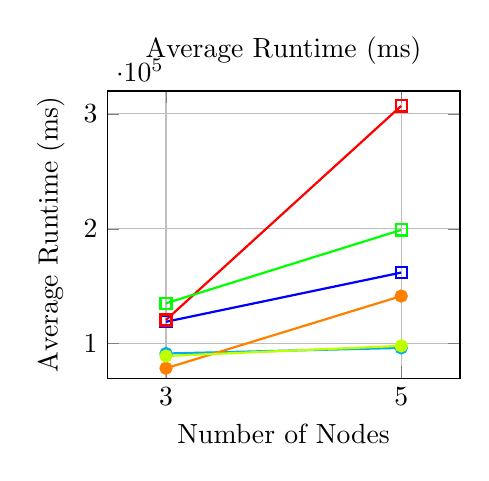
\begin{tikzpicture}
        \begin{axis}[
            title={Average Runtime (ms)},
            xlabel={Number of Nodes},
            ylabel={Average Runtime (ms)},
            xmin=2.5, xmax=5.5,
            ymin=70000, ymax=320000,
            xtick={3,5},
            width=0.5\textwidth,  
            grid=major,
        ]
        
        \addplot[
            color=cyan,
            mark=*,
            thick,
        ]
        coordinates {
            (3, 91423)
            (5, 96358)
        };
        
         \addplot[
            color=blue,
            mark=square,
            thick,
        ]
        coordinates {
            (3, 119080)
            (5, 161913)
        };

        \addplot[
            color=orange,
            mark=*,
            thick,
        ]
        coordinates {
            (3, 78625)
            (5, 141459)
        };
        
         \addplot[
            color=red,
            mark=square,
            thick,
        ]
        coordinates {
            (3, 120660)
            (5, 307010)
        };

        \addplot[
            color=lime,
            mark=*,
            thick,
        ]
        coordinates {
            (3, 89269)
            (5, 98119)
        };
        
         \addplot[
            color=green,
            mark=square,
            thick,
        ]
        coordinates {
            (3, 135186)
            (5, 199040)
        };

        \end{axis}
    \end{tikzpicture}
    \caption{Average Runtime (ms)}
    \label{fig:scenario1_plot}
\end{figure} 

\begin{figure}[h!]
    \centering
    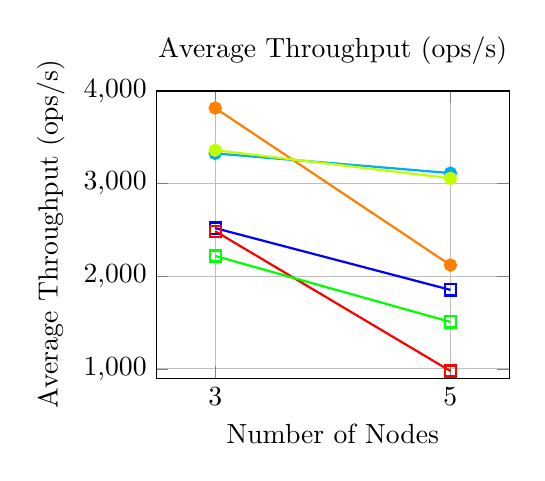
\begin{tikzpicture}
        \begin{axis}[
            title={Average Throughput (ops/s)},
            xlabel={Number of Nodes},
            ylabel={Average Throughput (ops/s)},
            xmin=2.5, xmax=5.5,
            ymin=900, ymax=4000,
            xtick={3,5},
            width=0.5\textwidth,  
            grid=major,
        ]
        
        \addplot[
            color=cyan,
            mark=*,
            thick,
        ]
        coordinates {
            (3, 3325.868606)
            (5, 3113.389651)
        };
        
         \addplot[
            color=blue,
            mark=square,
            thick,
        ]
        coordinates {
            (3, 2519.314746)
            (5, 1852.846899)
        };

        \addplot[
            color=orange,
            mark=*,
            thick,
        ]
        coordinates {
            (3, 3815.580286)
            (5, 2120.755837)
        };
        
         \addplot[
            color=red,
            mark=square,
            thick,
        ]
        coordinates {
            (3, 2486.325211)
            (5, 977.1668675)
        };

        \addplot[
            color=lime,
            mark=*,
            thick,
        ]
        coordinates {
            (3, 3360.62911)
            (5, 3057.511797)
        };
        
         \addplot[
            color=green,
            mark=square,
            thick,
        ]
        coordinates {
            (3, 2219.164706)
            (5, 1507.234727)
        };

        \end{axis}
    \end{tikzpicture}
    \caption{Average Throughput (ops/s)}
    \label{fig:scenario1_plot}
\end{figure} 

\begin{figure}[h!]
    \centering
    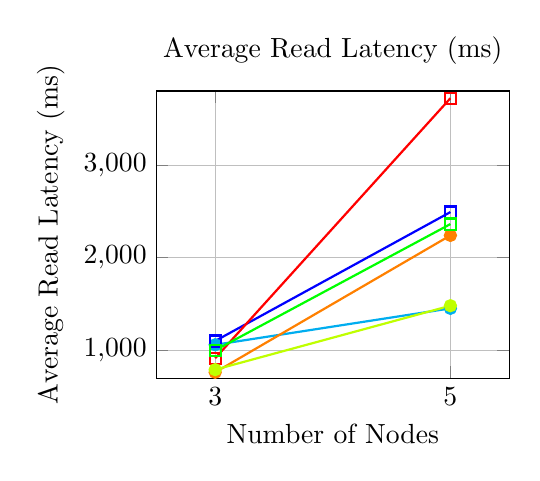
\begin{tikzpicture}
        \begin{axis}[
            title={Average Read Latency (ms)},
            xlabel={Number of Nodes},
            ylabel={Average Read Latency (ms)},
            xmin=2.5, xmax=5.5,
            ymin=700, ymax=3800,
            xtick={3,5},
            width=0.5\textwidth,  
            grid=major,
        ]
        
        \addplot[
            color=cyan,
            mark=*,
            thick,
        ]
        coordinates {
            (3, 1060.201079)
            (5, 1453.181125)
        };
        
         \addplot[
            color=blue,
            mark=square,
            thick,
        ]
        coordinates {
            (3, 1101.381226)
            (5, 2492.630748)
        };

        \addplot[
            color=orange,
            mark=*,
            thick,
        ]
        coordinates {
            (3, 763.2285631)
            (5, 2240.835886)
        };
        
         \addplot[
            color=red,
            mark=square,
            thick,
        ]
        coordinates {
            (3, 915.1947545)
            (5, 3721.425144)
        };

        \addplot[
            color=lime,
            mark=*,
            thick,
        ]
        coordinates {
            (3, 791.9283038)
            (5, 1481.94978)
        };
        
         \addplot[
            color=green,
            mark=square,
            thick,
        ]
        coordinates {
            (3, 1001.103408)
            (5, 2363.124744)
        };

        \end{axis}
    \end{tikzpicture}
    \caption{Average Read Latency (ms)}
    \label{fig:scenario1_plot}
\end{figure} 

\begin{figure}[h!]
    \centering
    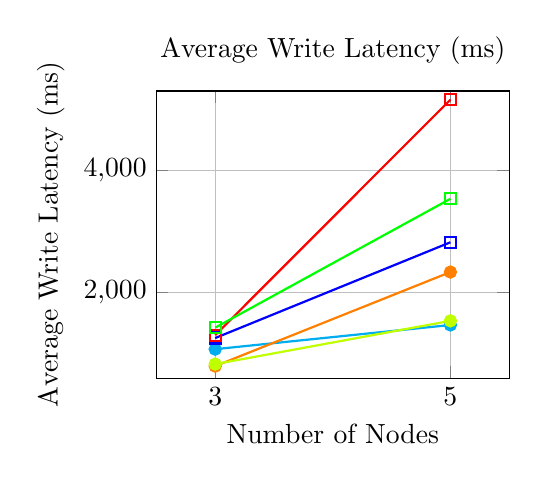
\begin{tikzpicture}
        \begin{axis}[
            title={Average Write Latency (ms)},
            xlabel={Number of Nodes},
            ylabel={Average Write Latency (ms)},
            xmin=2.5, xmax=5.5,
            ymin=600, ymax=5300,
            xtick={3,5},
            width=0.5\textwidth,  
            grid=major,
        ]
        
        \addplot[
            color=cyan,
            mark=*,
            thick,
        ]
        coordinates {
            (3, 1074.31284)
            (5, 1469.974975)
        };
        
         \addplot[
            color=blue,
            mark=square,
            thick,
        ]
        coordinates {
            (3, 1256.338213)
            (5, 2823.615044)
        };

        \addplot[
            color=orange,
            mark=*,
            thick,
        ]
        coordinates {
            (3, 797.221267)
            (5, 2336.257857)
        };
        
         \addplot[
            color=red,
            mark=square,
            thick,
        ]
        coordinates {
            (3, 1303.645599)
            (5, 5157.471893)
        };

        \addplot[
            color=lime,
            mark=*,
            thick,
        ]
        coordinates {
            (3, 829.5979688)
            (5, 1537.988751)
        };
        
         \addplot[
            color=green,
            mark=square,
            thick,
        ]
        coordinates {
            (3, 1426.374615)
            (5, 3534.90376)
        };

        \end{axis}
    \end{tikzpicture}
    \caption{Average Write Latency (ms)}
    \label{fig:scenario1_plot}
\end{figure} 

\pagebreak

\section{Conclusions}

We are pleased with our 3 implementations of the DLT/Replication stacks, as they address most of the challenges presented to us, with a blend of readable, extensible, and efficient code. In every experiment, the protocols performed robustly to any operations in the system, as expected, although performance suffered in some local tests, due to relatively low-powered hardware. \\

Not so surprisingly, the ABD Quorum algorithm performed rather well in these smaller scale, local tests, although, we suspect that with much higher node counts, the performance would rapidly decrease across all graphs. \\

As for the Paxos implementations, the Classic version functioned as expected during 3 node tests, but, quickly gave rise to performance problems when run with 5 nodes locally on a lower-powered laptop, as can be observed by every graph, Paxos Classic with a 10 KB Payload is unequivocally the worst outlier in every comparison. \\
Meanwhile, the Distinguished Learner version behaved quite well under the 5 node experiments, due to the much lower volume of messages across every transaction, so we suspect it can easily perform at a much higher node count.

\begin{acks}
  We would like to thank both our Distributed Systems Algorithms course professors, João Leitão and Alexander Davidson, for their support throughout these projects, both during and outside of classes. Their teaching styles were excellent throughout the semester, as professors who always pointed us in the right direction, without giving away too much, as to leave us room to develop our critical thinking.
  
  Of course, we also relied on provided lecture materials, along with some foundational research papers, which served as blueprints for our work, mainly regarding the Paxos Distinguished Learner protocol.
\end{acks}

\bibliographystyle{ACM-Reference-Format}
\bibliography{sample-base}
\nocite{*}
%%
%% The next two lines define the bibliography style to be used, and
%% the bibliography file.


\end{document}
\endinput
%%
%% End of file `sample-sigconf.tex'.
